%%%%% Package needed if some accented letters in the presentation
%%%%% -------------------------------------------------------------
\usepackage[utf8]{inputenc}


%%%%% Most beamer settings and other LaTeX commands
%%%%% are provided in the file below
%%%%% -----------------------------------------------------

%%%%% If to determine whether Czech or English version
%%%%% of a presentation is to be produced
%%%%% default = Czech
%%%%% ------------------------------------------------------
\newif\ifCZversion
\CZversiontrue

\ifCZversion\else\renewcommand{\uv}[1]{``#1''}\fi


%%%%% Included packages
%%%%% ----------------------------------------------------------
\usepackage[czech]{babel}
%\usepackage{lmodern}
%\usepackage[T1]{fontenc}
%\usepackage{textcomp}
\usepackage{natbib}         % zajištuje možnost odkazovat na literaturu
%\usepackage[natbib=true, bibstyle=authoryear, citestyle=authoryear-comp]{biblatex}
% stylem AUTOR (ROK), resp. AUTOR [ČÍSLO]
%\usepackage[nottoc]{tocbibind} % zajistí přidání seznamu literatury,

%\usepackage{array}
\usepackage{helvet}                       % font
\usepackage{amsmath}
\usepackage{amssymb}
\usepackage{amsfonts}       % matematické fonty
\usepackage{amsthm}         % sazba vět, definic apod.
\usepackage{dsfont} %pro indikátor
\usepackage{delarray}
\usepackage{multicol}
\usepackage{graphicx, fancybox}
\usepackage{psfrag}
\usepackage{fancyvrb}
\usepackage{eurosym}
\usepackage{bbding}
%\usepackage{bbold} %pro indikátor
\usepackage{bm}             % tučné symboly (příkaz \bm)
\usepackage{bbm}          % pro zdvojené !malá! písmena
\usepackage{mathtools} % pro použití multlined
\usepackage{multirow}
\usepackage[flushleft]{threeparttable} % footnotes pod tabulkou
\usepackage{dcolumn}        % lepší zarovnání sloupců v tabulkách
\usepackage{booktabs}       % lepší vodorovné linky v tabulkách
\usepackage{icomma}         % inteligetní čárka v matematickém módu
%\usepackage{paralist}       % lepší enumerate a itemize
%\usepackage[usenames]{xcolor}  % barevná sazba
% Moje přidané balíčky
\usepackage{comment} % prostředí pro komentování velkých bloků
%\usepackage{upgreek} % jiný font pro řecká písmena
%\usepackage{enumitem} % umožnuje lepší číslování v enumerate

%\usepackage{marvosym}
\usepackage{wasysym}
%\usepackage{ulem} %strikethrough \sout
%\usepackage{soul} %strikethrough \st

\usepackage[pdftex]{bookmark}


%%%%% Some LaTeX commands
%%%%% ----------------------------------------------------------
\renewcommand{\arraystretch}{1.2}


%%%%% Some colors and related commands
%%%%% ----------------------------------------------------------

%% Pantone 186 = "official" red of MFF
\definecolor{redmff}{rgb}{0.7892720,0.0651341,0.1455939}          

%% First level color = black
\definecolor{colOne}{rgb}{0,0,0}
\newcommand{\tOne}[1]{\textcolor{colOne}{#1}}
\newcommand{\tOneb}[1]{\textcolor{colOne}{\textbf{#1}}}
\newcommand{\tOnei}[1]{\textcolor{colOne}{\textit{#1}}}

%% Second level color = quite dark blue
\definecolor{colTwo}{rgb}{0,0,0.3}                
\newcommand{\tTwo}[1]{\textcolor{colTwo}{#1}}
\newcommand{\tTwob}[1]{\textcolor{colTwo}{\textbf{#1}}}
\newcommand{\tTwoi}[1]{\textcolor{colTwo}{\textit{#1}}}

%% Third level color = something between blue3 and blue4
\definecolor{colThree}{rgb}{0,0,0.7}              
\newcommand{\tThree}[1]{\textcolor{colThree}{#1}}
\newcommand{\tThreeb}[1]{\textcolor{colThree}{\textbf{#1}}}
\newcommand{\tThreei}[1]{\textcolor{colThree}{\textit{#1}}}

%% Color to alert (highlight) = MFF red
\definecolor{alertCol}{rgb}{0.7892720,0.0651341,0.1455939}
\newcommand{\tal}[1]{\alert{#1}}
\newcommand{\talb}[1]{\textbf{\alert{#1}}}
\newcommand{\tali}[1]{\textit{\alert{#1}}}

%% White
\newcommand{\tw}[1]{\textcolor{white}{#1}}
\newcommand{\twb}[1]{\textcolor{white}{\textbf{#1}}}
\newcommand{\twi}[1]{\textcolor{white}{\textit{#1}}}

%% Some other colors used somewhere
\definecolor{semiwhite}{gray}{0.98}
\definecolor{mffgray}{gray}{0.95}
\definecolor{semiblack}{gray}{0.5}
\definecolor{rred}{rgb}{0.5,0,0}
\definecolor{darkgreen}{rgb}{0,0.5,0}
\definecolor{lightgreen}{rgb}{0,0.8,0}

%%%%% Beamer stuff
%%%%% ----------------------------------------------------------
\mode<presentation> {
	
	%%% General theme of a presentation (some pre-specified themes)
	%%% ------------------------------------------------------------------
	%\usetheme{AnnArbor}
	\usetheme{CambridgeUS}
	%\usetheme{Warsaw}
	
	%%% Color schemes that will be used unless redefined below
	%%% ------------------------------------------------------------------
	%\usecolortheme{wolverine}
	%\usecolortheme{seagull}
	\usecolortheme{dolphin}
	%\usecolortheme{beaver}
	
	%%% Or do it yourself...
	%\useoutertheme{infolines}
	%\useoutertheme{miniframes}
	%\useoutertheme{shadow}
	%\useoutertheme{sidebar}
	%\useoutertheme{smoothbars}
	%\useoutertheme{smoothtree}
	%\useoutertheme{split}
	%\useoutertheme{tree}
	
	
	%%% Color schemes for different elements of a presentation
	%%% ---------------------------------------------------------
	
	%%% Uncomment the two rows below if some background file (layout) is to be used
	%%% on all slides
	%\usebackgroundtemplate{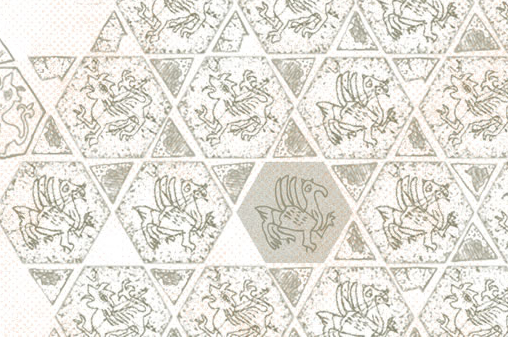
\includegraphics[width=\paperwidth, height=\paperheight]{./fig/BackgroundRotunda}}
	%\setbeamercolor{background canvas}{bg=}                                                             
	
	%%% Setting for "standard" slides
	%%% - must be commented if background file used
	%\setbeamertemplate{background canvas}[vertical shading][bottom=semiwhite, top=white, middle=semiwhite!50!white]
	%\setbeamercolor{background canvas}{bg=white}                           %% NO EFFECT WHEN \setbeamertemplate{background canvas} WAS USED
	
	%%% Colors of frametitle, normal, alerted and math texts
	%\setbeamercolor{frametitle}{fg=white, bg=redmff}
	%\setbeamercolor{normal text}{fg=black}
	%\setbeamercolor{alerted text}{fg=redmff}
	\setbeamercolor{math text inlined}{fg=colTwo}
	\setbeamercolor{math text displayed}{fg=colTwo}
	
	%%% Colors for some special boxes defined below
	\setbeamercolor{mffboxcol}{fg=colTwo, bg=mffgray}
	\setbeamercolor{mffboxcolupper}{fg=white, bg=redmff}
	\setbeamercolor{vetacolupper}{fg=white, bg=darkgreen}
	\setbeamercolor{tvrzcolupper}{fg=white, bg=lightgreen}
	\setbeamercolor{definicecolupper}{fg=white, bg=blue}
	\setbeamercolor{algcolupper}{fg=black, bg=pink}
	
	%%% Set serif font (patkové písmo) in mathematics
	%%% ------------------------------------------------
	%\usefonttheme[onlymath]{serif}
	
	%%% Itemize style (rectangles instead of bullets)
	%%% ------------------------------------------------
	%\useinnertheme{rectangles}
	
	%%% Default content of a header of each slide
	%%% (currently nothing)
	%%% ------------------------------------------------
	%\setbeamertemplate{headline}{}
	
	%%% Default content of a foot of each slide
	%%% ------------------------------------------------
	%\setbeamercolor{page number in head/foot}{fg=black, bg=white}
	\setbeamertemplate{footline}{
		\hspace*{1em}
		\begin{beamercolorbox}{white}
			\vskip1pt
			\tOne{\rule{\textwidth}{1pt}}
			\vskip2pt
			
			%%% Foot containing (a) page number/total number of pages, (b) name, (c) short title of presentation
			{\small \tOne{\insertframenumber}\textcolor{semiblack}{/\inserttotalframenumber}}\hspace{2em}
			\tOne{\footnotesize \insertauthor}\hfill
			%\tOne{\footnotesize\insertshorttitle\hspace{3em}}
			{\usebeamercolor[fg]{structure} \footnotesize\insertshorttitle\hspace{3em}}
			
			%%% Foot containing (a) page number/total number of pages, (b) name, (c) short section title
			%{\small \tOne{\insertframenumber}\textcolor{semiblack}{/\inserttotalframenumber}}\hspace{1em}
			%\tOne{\footnotesize \insertauthor}\hfill
			%\textcolor{redmff}{\footnotesize\thesection. \insertsection\hspace{3em}}
			
			\hspace*{3.5em}
			\vskip3pt
		\end{beamercolorbox}
	}
	
	%%% Title page
	%%% -------------------
	\setbeamertemplate{title page}{
		%\vspace*{-0.5em}
		\begin{center}
			\ifCZversion
			
\includegraphics[height=35mm]{./fig/logotyp_fakulty_rgb1}
			\else
			
\includegraphics[height=35mm]{./fig/logotyp_fakulty_rgb2}
			\fi
			
			\bigskip
			\textcolor{black}{\normalsize\bfseries \insertauthor} \\[0.5ex]
			\textcolor{black}{\small \insertinstitute}
			
			\bigskip
			{\usebeamercolor[fg]{structure}{\Large\bfseries \inserttitle}}
			
			\medskip
			{\usebeamercolor[fg]{structure}{\large\insertsubtitle}}
			
			\bigskip
			\textcolor{colTwo}{\small \insertdate}
		\end{center}
	}    
	
	%%% Switch-off/on foot with navigation symbols    
	%%% -----------------------------------------------
	% \setbeamertemplate{navigation symbols}{}
	\usenavigationsymbolstemplate{}
	
	%%% Left and right margin
	%%% --------------------------------
	%\setbeamersize{text margin left=1cm}
	%\setbeamersize{text margin right=1cm}
	
	
	%%% Use of a logo on each slide
	%%% (not really recommended, so commented)
	%\logo{
\includegraphics[height=1.5cm, width=1.5cm]{./fig/mff_logo}}
}


%%%%% Commands to produce slides at the beginning of each section
%%%%% --------------------------------------------------------------
\renewcommand{\thesection}{\arabic{section}}
\newcommand{\framesection}{
	\begin{frame} %[plain]
		\vspace*{2em}
		\begin{center}\Large
			\ifCZversion Oddíl \thesection \else Section \thesection \fi
		\end{center}
		\begin{center}\color{rred}\Large
			\insertsection
		\end{center}
	\end{frame}
}



%%%%% Style for software related stuff
%%%%% ----------------------------------------------------------
\newcommand{\Rko}{
\includegraphics[width=5.094mm, height=3.876mm]{./fig/Rlogo}}
\newcommand{\Rfun}[1]{\textcolor{redmff}{\texttt{#1}}}

\DefineVerbatimEnvironment{Rin}{Verbatim}{formatcom=\color{redmff}, fontsize=\scriptsize, frame=single, framerule=1pt, framesep=2pt}
\DefineVerbatimEnvironment{Rout}{Verbatim}{formatcom=\color{blue}, fontsize=\scriptsize, frame=single, framerule=1pt, framesep=2pt}


%%%%% Boxes
%%%%% ----------------------------------------------------------
\newcommand{\mffbox}[2][0pt]{%
	\begin{beamercolorbox}[center, sep=#1, rounded=true, shadow=true]{mffboxcol}
		#2
	\end{beamercolorbox}
}

\newcommand{\mffboxshort}[2][0pt]{%
	\begin{beamercolorbox}[center, wd=0.5\paperwidth, sep=#1, rounded=true, shadow=true]{mffboxcol}
		#2
	\end{beamercolorbox}
}

\newcommand{\mffboxTitle}[2]{%
	\begin{beamerboxesrounded}[lower=mffboxcol, upper=mffboxcolupper, shadow=true]{#1}
		#2
	\end{beamerboxesrounded}
}

\newcommand{\veta}[2]{%
	\begin{beamerboxesrounded}[lower=mffboxcol, upper=vetacolupper, shadow=true]{
			\ifCZversion \textbf{Věta} #1 \else \textbf{Theorem} #1 \fi}
		#2
	\end{beamerboxesrounded}
}

\newcommand{\tvrz}[2]{%
	\begin{beamerboxesrounded}[lower=mffboxcol, upper=tvrzcolupper, shadow=true]{
			\ifCZversion \textbf{Tvrzení} #1 \else \textbf{Lemma} #1 \fi}
		#2
	\end{beamerboxesrounded}
}

\newcommand{\definice}[1]{%
	\begin{beamerboxesrounded}[lower=mffboxcol, upper=definicecolupper, shadow=true]{
			\ifCZversion \textbf{Definice} #1 \else \textbf{Definition} #1 \fi}
		#1
	\end{beamerboxesrounded}
}

\newcommand{\alg}[2]{%
	\begin{beamerboxesrounded}[lower=mffboxcol, upper=algcolupper, shadow=true]{
			\ifCZversion \textbf{Algoritmus} #1 \else \textbf{Algorithm} #1 \fi}
		#2
	\end{beamerboxesrounded}
}


%%%%% Some constructions for displayed math
%%%%% ----------------------------------------------------------
\newcommand{\dmath}[2][-1.4em]{%
	\begin{beamercolorbox}[center, sep=#1, rounded=true, shadow=true]{mffboxcol}
		\begin{displaymath}
			#2
		\end{displaymath}
	\end{beamercolorbox}
}

\newcommand{\dalign}[2][-1.4em]{%
	\begin{beamercolorbox}[center, sep=#1, rounded=true, shadow=true]{mffboxcol}
		\begin{align*}
			#2
		\end{align*}
	\end{beamercolorbox}
}

\newcommand{\dgather}[2][-1.4em]{%
	\begin{beamercolorbox}[center, sep=#1, rounded=true, shadow=true]{mffboxcol}
		\begin{gather*}
			#2
		\end{gather*}
	\end{beamercolorbox}
}

%%%%% \ifCZversion is defined inside MFF_Present.sty
%%%%% to distinguish between Czech and English presentations
%%%%% ------------------------------------------------------
%\CZversiontrue       %% for presentations in Czech (Slovak)
\CZversionfalse      %% for presentations in English


%%%%% Uncomment appropriate choice below if you wish to create
%%%%% notes for audience having 2 or 4 slides on each (A4) page.
%%%%% -------------------------------------------------------------
\usepackage{pgfpages}
%\pgfpagesuselayout{4 on 1}[a4paper, landscape, border shrink=5mm]
%\pgfpagesuselayout{2 on 1}[a4paper, border shrink=5mm]


%%%%% My added packages
\usepackage{animate}
\usepackage{tikz}
\usepackage{algpseudocode}
\usepackage{algorithmicx} % algorithm and algorithmic environment
\usepackage{algorithm}

%%%%% Basic settings of the document
%%%%% (will be automatically used to create a title page, foots etc.)
%%%%% --------------------------------------------------------------------

%%% Main title
%%% - short and long version
%%%   --> will appear on place where \inserttitle and \insertshorttitle commands used
%%%   --> if the full title is short enough, both short and long versions might be the same
\title[Model-based Clustering of Multivariate Longitudinal Data of a Mixed Type]{%
	Model-based Clustering of Multivariate Longitudinal Data of a Mixed Type}

%%% Subtitle (comment it if you do not want to have it)
%%%   --> will appear on place where \insertsubtitle and \insertshortsubtitle commands used
%\subtitle[]{}

%%% Author
%%% - as "short" version, link to the author's webpage is used
%%%   (e.g., e-mail is also a useful alternative)
%%%   --> will appear on places where \insertauthor and \insertshortauthor commands used
\author[Jan Vávra]{%
	Jan Vávra}

%%% Author's affiliation
%%% - can be fully commented for defense presentation
%%%   --> will appear on places where \insertinstitute and \insertshortinstitute commands used
\institute[DPMS]{%
	Department of Probability and Mathematical Statistics}

%%% Date of presentation
%%% - replace it by real date in case of a defense presentation
%%%   --> will appear on places where \insertdate and \insertshortdate commands used
\date[9.1.2023]{%
	9th January 2023 \qquad Doctoral thesis defence}

\newcommand{\jdedonekonecna}[1]{\stackrel{#1\rightarrow\infty}{\longrightarrow}}
\newcommand{\necojdenekam}[2]{\stackrel{#1\rightarrow #2}{\longrightarrow}}

%%% prostor reálných, resp. přirozených čísel
\newcommand{\R}{\mathbb{R}}
\newcommand{\N}{\mathbb{N}}

%%% Užitečné operátory pro statistiku a pravděpodobnost
\DeclareMathOperator{\pr}{\mathsf{P}}
\DeclareMathOperator{\E}{\mathsf{E}}
\DeclareMathOperator{\logit}{\mathrm{logit}}
\DeclareMathOperator{\softmax}{\mathrm{softmax}}
\newcommand{\SE}{\mathsf{SE}}
\newcommand{\SEP}{\mathsf{SEP}}
\newcommand{\SoS}{\mathsf{SS}}
\newcommand{\SSE}{\mathsf{SSE}}
\newcommand{\MSE}{\mathsf{MSE}}
\newcommand{\RMSE}{\mathsf{RMSE}}
\newcommand{\MAE}{\mathsf{MAE}}
\newcommand{\MAPE}{\mathsf{MAPE}}
\DeclareMathOperator{\var}{\mathsf{var}}
\DeclareMathOperator{\cov}{\mathsf{cov}}
\DeclareMathOperator{\corr}{\mathsf{corr}}
\DeclareMathOperator{\sd}{\mathsf{sd}}
\DeclareMathOperator{\med}{\mathsf{med}}
\DeclareMathOperator{\diag}{\mathsf{diag}}
\DeclareMathOperator{\rank}{\mathsf{rank}}
\DeclareMathOperator{\Tr}{\mathsf{Tr}}
\DeclareMathOperator*{\argmin}{\mathrm{arg\,min}}
\DeclareMathOperator*{\argmax}{\mathrm{arg\,max}}
\renewcommand{\det}{\mathsf{det}}
\renewcommand{\vec}{\mathsf{vec\,}}
\renewcommand{\mod}{\mathsf{mod\,}} % modus
\renewcommand{\mid}{\;\middle\vert\!}

%%% Příkaz pro transpozici vektoru/matice
\newcommand{\T}[1]{#1^\top}

%%% Vychytávky pro matematiku
\newcommand{\goto}{\rightarrow}
\newcommand{\gotop}{\stackrel{P}{\longrightarrow}}
\newcommand{\maon}[1]{o(n^{#1})}
\newcommand{\abs}[1]{\left|{#1}\right|}
\newcommand{\dint}{\int_0^\tau\!\!\int_0^\tau}
\newcommand{\isqr}[1]{\frac{1}{\sqrt{#1}}}
%\newcommand{\indikator}{\mathds{1}} %%svázáno s balíčkem dsfont %% možnost nahradit \mathbb{1} ale s balíčkem bbold
\newcommand{\indikator}{\mathbb{I}}
%\newcommand{\indikator}{\mathbb{1}} %%svázáno s balíčkem bbold %% možnost nahradit \mathds{1} ale s balíčkem dsfont
\newcommand{\jednotky}{\bm 1}
\newcommand{\poloz}{\stackrel{!}{=}}
%\newcommand{\Rko}{\textcolor{blue}{\textbf{R}}} %% symbol pro statistický software R
%\newcommand{\Rko}{
\includegraphics[width=5.094mm, height=3.876mm]{./fig/Rlogo}}
\newcommand{\Ccko}{\raisebox{-0.35ex}[0pt]{
\includegraphics[width=3.5mm, height=3.5mm]{./fig/Clogo2}}}
\newcommand{\RStan}{\raisebox{-0.35ex}[0pt]{
\includegraphics[width=3.5mm, height=3.5mm]{./fig/RStanlogo}}}

%%% Probability distributions
\newcommand{\norm}[2]{\mathsf{N}\left(#1, \,#2 \right)} %normal 1=E,2=var
\newcommand{\knorm}[3]{\mathsf{N}_{#1}\left(#2, \,#3 \right)} %MV normal 1=dim k, 2=E, 3=var
\newcommand{\mnorm}[4]{\mathsf{N}_{#1\times #2}\left(#3, \,#4\right)} %matrix normal 1=nrow, 2=ncol, 3=E, 4=var of vec(X)

\newcommand{\Tnorm}[4]{\mathsf{TN}\left(#1, \,#2, \,#3, \,#4 \right)} %normal 1=E, 2=var, 3=lower, 4=upper


\newcommand{\gammadist}[2]{\Gamma\left(#1, #2 \right)} %Gamma distribution 1=shape a, 2=rate lambda
\newcommand{\W}[3]{\mathsf{W}_{#1}\left(#2, #3 \right)} %Wishart 1=dim, 2=scale matrix, 3=df
\newcommand{\IW}[3]{\mathsf{IW}_{#1}\left(#2, #3 \right)} %Inverse Wishart 1=dim, 2=scale matrix, 3=df

\newcommand{\lognorm}[2]{\mathsf{LN}\left(#1, #2 \right)} %log-normal 1=ElogX, 2=varlogX
\newcommand{\Bern}[1]{\mathsf{Bernoulli}\left(#1\right)} %alternative = bernoulli 1=prob
\newcommand{\Bi}[2]{\mathsf{Bi}\left(#1, #2 \right)} %binomial 1=n(observations), 2=prob(succes)
\newcommand{\Mult}[3]{\mathsf{Mult}_{#1}\left(#2, #3 \right)} %multinomial 1=K (ngroups), 2=n(observations), 3=probs
\newcommand{\Geom}[1]{\mathsf{Geom}\left(#1 \right)} %geometric 1=prob succes
\newcommand{\Pois}[1]{\mathsf{Pois}\left(#1 \right)} %Poisson 1=lambda
\newcommand{\Linmodel}[2]{\left(#1, #2\right)} %Linear model 1=E, 2=var
\newcommand{\NLinmodel}[2]{\mathsf{N}\left(#1, #2\right)} %Normal linear model 1=E, 2=var

\newcommand{\Chisq}[1]{\chi_{#1}^2} %Chi square 1=df
\newcommand{\st}[1]{\mathsf{t}_{#1}} %Student 1=df
\newcommand{\F}[2]{\mathsf{F}_{#1, #2}} %Fisher-Snedecor 1=df1, 2=df2

\newcommand{\Dirac}[1]{\mathsf{D}_{\{#1\}}} %Dirac distribution - concentrated in #1
\newcommand{\Unif}[2]{\mathsf{Unif}\left(#1, #2\right)} %1-min, 2 - max
\newcommand{\Unifoo}[2]{\mathsf{Unif}\left(#1, #2\right)} %Uniform() 1=min, 2=max
\newcommand{\Unifoc}[2]{\mathsf{Unif}\left(\left.#1, #2\right]\right.} %Uniform(] 1=min, 2=max
\newcommand{\Unifco}[2]{\mathsf{Unif}\left[\left.#1, #2\right)\right.} %Uniform[) 1=min, 2=max
\newcommand{\Unifcc}[2]{\mathsf{Unif}\left[#1, #2\right]} %Uniform[] 1=min, 2=max
\newcommand{\Unifset}[1]{\mathsf{Unif}\left\{#1\right\}} %Uniform{} 1=values
\newcommand{\Beta}[2]{\mathsf{Beta}\left(#1, #2\right)} %Beta 1-alpha, 2 - beta
\newcommand{\Betafun}[2]{\mathsf{B}\left(#1, #2\right)} %Beta function 1-alpha, 2 - beta
\newcommand{\Dir}[2]{\mathsf{Dir}_{#1}\left(#2\right)} %Dirichlet distribution 1=dim, 2=alphas

%%% shortcuts
\newcommand{\Num}{\mathsf{Num}}
\newcommand{\Poi}{\mathsf{Poi}}
\newcommand{\Bin}{\mathsf{Bin}}
\newcommand{\Ord}{\mathsf{Ord}}
\newcommand{\Cat}{\mathsf{Cat}}
\newcommand{\OB}{\mathsf{OB}}
\newcommand{\NN}{\mathsf{N}}
\newcommand{\PP}{\mathsf{P}}
\newcommand{\BB}{\mathsf{B}}
\newcommand{\OO}{\mathsf{O}}
\newcommand{\CC}{\mathsf{C}}
\newcommand{\RNum}{\mathcal{R}^{\Num}}
\newcommand{\RPoi}{\mathcal{R}^{\Poi}}
\newcommand{\RBin}{\mathcal{R}^{\Bin}}
\newcommand{\ROrd}{\mathcal{R}^{\Ord}}
\newcommand{\RCat}{\mathcal{R}^{\Cat}}
\newcommand{\ROB}{\mathcal{R}^{\OB}}

\newcommand{\GARCH}[2]{\mathsf{GARCH}\left(#1, #2 \right)} %1-řád autoregrese vůči epsilonu a 2- řád autoregrese vůči sigma_t^2

\newcommand{\selG}{4}
\newcommand{\selch}{4}


%%% Vychytávky pro tabulky
\newcommand{\pulrad}[1]{\raisebox{1.5ex}[0pt]{#1}}
\newcommand{\mc}[1]{\multicolumn{1}{c}{#1}}
\setlength{\tabcolsep}{5pt}

%%% Symbol z \item commandu
\newcommand\mytextbullet{\leavevmode%
	\usebeamertemplate{itemize item}\hspace{.5em}}


%%% Barvy
\definecolor{amber}{rgb}{1.0, 0.75, 0.0}
\definecolor{amber(sae/ece)}{rgb}{1.0, 0.49, 0.0}
\definecolor{burntorange}{rgb}{0.8, 0.33, 0.0}
\definecolor{fluorescentorange}{rgb}{1.0, 0.75, 0.0}
\definecolor{chromeyellow}{rgb}{1.0, 0.65, 0.0}
\definecolor{chartreuse(web)}{rgb}{0.5, 1.0, 0.0}
\definecolor{green-yellow}{rgb}{0.68, 1.0, 0.18}
\definecolor{forestgreen(web)}{rgb}{0.13, 0.55, 0.13}
\definecolor{cream}{rgb}{1.0, 0.99, 0.82}